% The three ways of enlarging a cycle in the proof of Jackson's theorem.
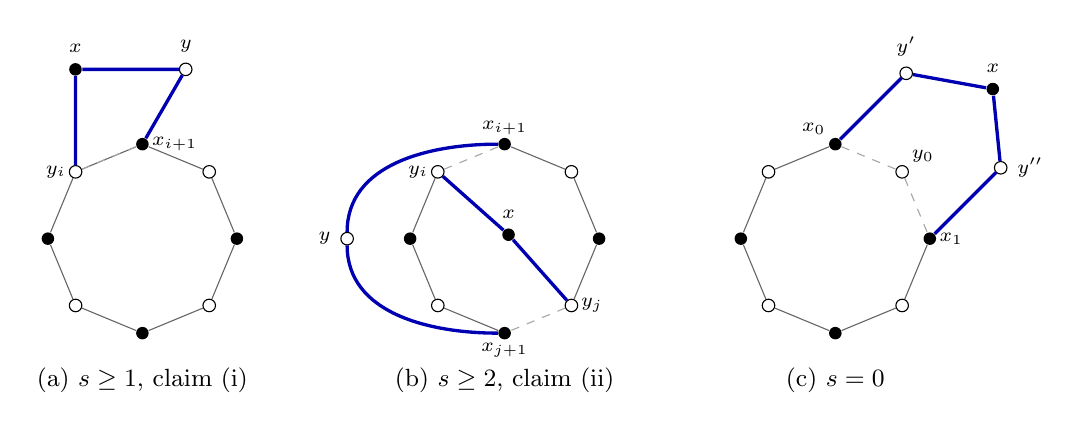
\begin{tikzpicture}[
  xv/.style={circle, fill=black, inner sep=1.6pt},
  yv/.style={circle, draw=black, fill=white, inner sep=1.6pt},
  old/.style={black!60}, new/.style={very thick, blue!70!black},
  gone/.style={black!35, dashed}, lab/.style={font=\scriptsize}]
\begin{scope}
\foreach \k/\t in {0/xv,1/yv,2/xv,3/yv,4/xv,5/yv,6/xv,7/yv}
  \node[\t] (a\k) at ({90-45*\k}:1.2) {};
\draw[old] (a1)--(a2)--(a3)--(a4)--(a5)--(a6)--(a7)--(a0)--(a1);
\draw[gone] (a7)--(a0);
\node[xv, label={[lab]above:$x$}] (x) at (-0.85,2.15) {};
\node[yv, label={[lab]above:$y$}] (y) at (0.55,2.15) {};
\draw[new] (a7) -- (x) -- (y) -- (a0);
\node[lab, left] at (a7) {$y_i$};
\node[lab, right] at (a0) {$x_{i+1}$};
\node[font=\small] at (0,-1.8) {(a) $s\ge1$, claim (i)};
\end{scope}
\begin{scope}[xshift=4.6cm]
\foreach \k/\t in {0/xv,1/yv,2/xv,3/yv,4/xv,5/yv,6/xv,7/yv}
  \node[\t] (b\k) at ({90-45*\k}:1.2) {};
\draw[old] (b0)--(b1)--(b2)--(b3);
\draw[old] (b4)--(b5)--(b6)--(b7);
\draw[gone] (b7)--(b0);
\draw[gone] (b3)--(b4);
\node[xv, label={[lab]above:$x$}] (x) at (0.05,0.05) {};
\node[yv, label={[lab]left:$y$}] (y) at (-2.0,0) {};
\draw[new] (b7) -- (x) -- (b3);
\draw[new] (b0) to[out=180, in=90] (y);
\draw[new] (y) to[out=-90, in=180] (b4);
\node[lab, left] at (b7) {$y_i$};
\node[lab, above] at (b0) {$x_{i+1}$};
\node[lab, right] at (b3) {$y_j$};
\node[lab, below] at (b4) {$x_{j+1}$};
\node[font=\small] at (0,-1.8) {(b) $s\ge2$, claim (ii)};
\end{scope}
\begin{scope}[xshift=8.8cm]
\foreach \k/\t in {0/xv,1/yv,2/xv,3/yv,4/xv,5/yv,6/xv,7/yv}
  \node[\t] (c\k) at ({90-45*\k}:1.2) {};
\draw[old] (c2)--(c3)--(c4)--(c5)--(c6)--(c7)--(c0);
\draw[gone] (c0)--(c1)--(c2);
\node[xv, label={[lab]above:$x$}] (x) at (2.0,1.9) {};
\node[yv, label={[lab]above:$y'$}] (y1) at (0.9,2.1) {};
\node[yv, label={[lab]right:$y''$}] (y2) at (2.1,0.9) {};
\draw[new] (c0) -- (y1) -- (x) -- (y2) -- (c2);
\node[lab, above left] at (c0) {$x_0$};
\node[lab, right] at (c2) {$x_1$};
\node[lab, above right] at (c1) {$y_0$};
\node[font=\small] at (0,-1.8) {(c) $s=0$};
\end{scope}
\end{tikzpicture}
